\chapter{Conceitos Básicos}\label{ch:conceitos-basicos}

% FIXME: adicionar mais referências.
% FIXME: mais conceitos básicos e de forma didática.
% FIXME: Novamente use a estratégia “funil”.
% Qual área lida com o problema?
% Quais métodos são aplicáveis, aí direciona para o que vc vai apresentar,
% justificando e dando uma visão geral do capítulo.
% Só aí inicia a seção 2.1

Antes de estudar o problema, são necessários alguns conceitos básicos e definição formal de termos
importantes para a área de Pesquisa Operacional e otimização.
Pesquisa Operacional pode ser entendida como o estudo e a aplicação de métodos científicos para
tomada de decisões em problemas complexos~\cite[p.IX]{arenales}.
Ela permite modelar, analisar e solucionar tais problemas de modo, geralmente, satisfatório.

Neste capítulo é explicado sobre modelos de otimização (\autoref{sec:modelos-de-otimizacao})
e seus tipos (\autoref{sec:tipos-de-modelo}), além de algumas definições sobre otimização,
finalizando com a diferença entre métodos heurísticos e exatos
(\cref{sec:metodos-exatos-heuristicos}).
O problema de empacotamento de retângulos (detalhado no \Cref{ch:problema-de-empacotamento}),
alvo deste estudo, é determinístico e pode ser modelado utilizando programação linear inteira
mista~\cite{wolsey2020integer}.
No trabalho, o problema será explorado do ponto de vista heurístico, com o método apresentado no
\Cref{ch:bottom-left}.

\section{Modelos de otimização e definições}\label{sec:modelos-de-otimizacao}
% FIXME: adicionar referência

Modelos de otimização são aproximações da realidade, representam o problema de maneira simples
e objetiva, usando restrições.
De forma geral, um modelo de otimização busca minimizar ou maximizar uma função $f(x)$ com $x$
obedecendo algumas restrições.
Pode-se então representar o modelo do seguinte modo:

\[
    \min\!/\!\max f(x), x \in \mathcal{X}.
\]


Onde

\begin{itemize}
    \item $x$: variáveis de decisão, $x = (x_1, x_2, \dots, x_n)$.
    \item $\mathcal{X}$: conjunto factível ou domínio, possui todas as soluções viáveis para o problema.
    \item $f(x)$: função objetivo, a qual determinará o critério de escolha da solução.
\end{itemize}

A seguir serão dadas as definições de quatro expressões que aparecem com frequência no estudo de
problemas de otimização.

Uma solução $x'$ é \textbf{factível} somente se satisfaz todas as restrições dadas ao problema,
ou seja, $x' \in \mathcal{X}$.
Existem casos onde o problema não tem solução, possivelmente por muitas restrições terem sido
aplicadas.
Isso é chamado \textbf{problema infactível} e $\mathcal{X} = \emptyset$.
Se para toda solução for possível encontrar outra melhor o problema é dito \textbf{ilimitado}.

Uma solução $x'$ é \textbf{ótima} somente se for \textbf{factível} e possuir resultado melhor,
ou igual, que as demais soluções, isto é, $f(x') \le f(x), \forall x \in \mathcal{X}$ (caso seja um
problema de maximização é necessário substituir “$\le$” por “$\ge$”).
Importante observar que existe somente solução ótima se o problema não for infactível nem ilimitado.

Usando o problema da mochila como exemplo, onde se busca maximizar o valor dos itens alocados
sem que seus pesos ultrapassem a capacidade da mochila~\cite{exact-solution-techniques},
um modelo possível é:

\[
    \max { \sum_{i \in I} v_{i} x_{i}: \sum_{i \in I} w_{i} x_{i} \leq C}
\]


Em que $I$ é um conjunto de itens, $v_{i}$ e $w_{i}$ são, respectivamente o valor e o peso do item
$i \in I$, $C$ é a capacidade da mochila e $x_{i}$ são variáveis binárias indicando se o
item foi escolhido para mochila ou não.

O problema não é ilimitado, já que a melhor solução (solução ótima) é ocupar toda a capacidade $C$
da mochila, caso seja possível com os itens $I$.
Qualquer solução que não ultrapasse o limite da mochila é factível.
O problema só será considerado infactível caso não seja possível alocar pelo menos um item, ou seja,
todos os itens possuírem peso $w_i > C$.

\section{Tipos de Modelo}\label{sec:tipos-de-modelo}
% TODO: adicionar figuras

É importante saber diferenciar os modelos devido ao método de resolução que varia para cada um deles.

\subsection{Modelo Linear × Não-linear}\label{subsec:modelo-linear}


Modelos lineares possuem como função objetivo uma função linear e todas as restrições também são lineares.
Exemplos:

\begin{itemize}
    \item $f(x) = ax + b$.
    \item $f(x_1, x_2) = x_1 + x_2 - 5$.
\end{itemize}

Já os não-lineares não obedecem essa regra, podendo ter suas variáveis se multiplicando ou funções trigonométricas e logarítmicas.
Exemplos:

\begin{itemize}
    \item $f(x_1, x_2) = x_1^2 + x_2^2$.
    \item $f(x_1, x_2) = \tan(x_1 + x_2)$.
\end{itemize}

\begin{figure}[H]
    \centering
    \caption{Exemplo de modelo linear e não-linear.}
    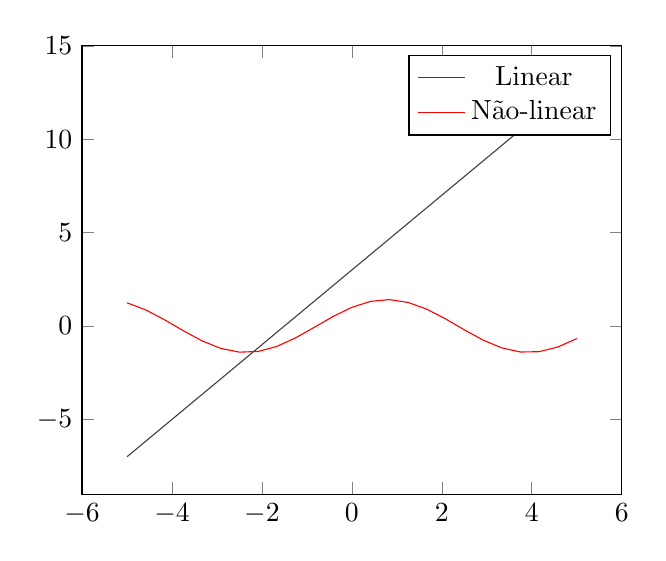
\begin{tikzpicture}
    \begin{axis}
        \addplot[darkgray] {2*x + 3};
        \addplot[red] {cos(deg(x)) + sin(deg(x))};
        \legend{Linear, Não-linear}
    \end{axis}
\end{tikzpicture}

    \label{fig:linear-nao-linear}
    \fonte{feito pelo autor.}
\end{figure}


\subsection{Modelo Contínuo × Discreto}\label{subsec:modelo-continuo-x-discreto}

Um modelo é contínuo quando sua região factível é contínua, ou seja, dado um ponto dessa região todos os seus vizinhos também serão uma solução.
Modelos discretos não possuem seu domínio contínuo.
A \autoref{fig:continuo-discreto} mostra um gráfico com exemplos de um modelo contínuo e outro discreto.

\begin{figure}[!htb]
    \centering
    \caption{Exemplo de modelo contínuo e discreto.}
    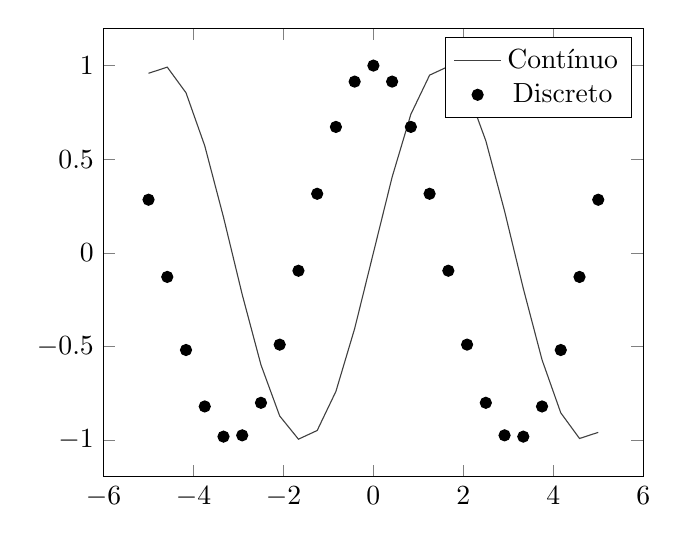
\begin{tikzpicture}
    \begin{axis}
        \addplot[darkgray] {sin((deg(x))};
        \addplot[black, only marks] {cos(deg(x))};
        \legend{Contínuo, Discreto}
    \end{axis}
\end{tikzpicture}

    \label{fig:continuo-discreto}
    \fonte{feito pelo autor.}
\end{figure}


\subsection{Modelo Determinístico × Estocástico}\label{subsec:modelo-deterministico-x-estocastico}

Em modelos determinísticos seus dados são conhecidos, enquanto os estocásticos possuem uma
incerteza quanto aos dados.

\subsection{Tipos de Programação}\label{subsec:tipos-de-programacao}

Com base nas categorias de modelo é possível também dividir métodos de programação (planejamento)
para sua solução.
\citeauthor*{hillier1967introduction} traz alguns exemplos algoritmos de para os tipos de programação.

\begin{itemize}
    \item Linear: modelo linear contínuo determinístico.
    Algoritmos importantes para essa classe de problemas são: o algoritmo Simplex
    e algoritmos de pontos interiores.
    \item Inteira: modelo linear discreto determinístico.
    Aqui se destacam os algoritmos \textit{branch-and-bound} e \textit{branch-and-cut}.
    \item Estocástica: modelo linear contínuo estocástico.
    Alguns métodos para solução podem se basear em simulação dos eventos aleatórios envolvidos.
    \item Não-linear: modelo não-linear contínuo determinístico.
    Os algoritmos para solução de problemas não lineares podem ser baseados em gradiente,
    mas com frequência dependem bastante do problema a ser resolvido.
\end{itemize}

\section{Métodos Exatos × Heurísticos}\label{sec:metodos-exatos-heuristicos}
% TODO: falar mais sobre heurísticas e como escapar de ótimos locais.
% FIXME: referências

Métodos exatos sempre vão garantir a solução ótima para o problema, porém encontrar
tal solução pode requerer grande tempo e/ou muitos recursos computacionais.
Já heurísticas buscam por soluções factíveis e são geralmente usadas em problemas de grande porte.

Um dos métodos exatos mais conhecidos é o algoritmo \textit{branch-and-bound}, ele realiza a
enumeração implícita das soluções viáveis de um problema de programação linear inteira mista,
mantendo valores para os limitantes inferior e superior de um problema de otimização.
O algoritmo termina sua execução quando ambos os limitantes se igualam, garantindo a otimalidade
da solução.
Detalhes do algoritmo \textit{branch-and-bound} e outros para problemas de programação inteira,
como \textit{branch-and-cut} e planos de corte podem ser vistos em \citeauthoryear{wolsey2020integer}.

Como o problema de empacotamento de retângulos é NP-difícil e o principal interesse é em instâncias
de médio e grande porte, utilizar um método exato seria bastante desafiador e, provavelmente,
não seria possível obter um resultado em tempo hábil devido aos recursos computacionais disponíveis.
Portanto, métodos heurísticos serão usados, já que eles tendem a diminuir a demanda computacional,
porém não garantem otimalidade da solução resultante.

Soluções heurísticas tipicamente alternam entre explorar o espaço de busca de forma mais ampla
e se concentrar em uma vizinhança de uma solução viável já encontrada.
Por isso, em geral, uma heurística garante apenas a otimalidade local da solução.
Para escapar de ótimos locais e buscar atingir um resultado melhor, mecanismos de fuga são usados.
Alguns exemplos desses mecanismos são o \textit{multi-start} e o \textit{simulated annealing}~\cite{
    firat2020effective,rakotonirainy2020improved,hopper2001empirical}.

Continuando o exemplo do problema da mochila~(\cref{sec:modelos-de-otimizacao}), uma heurística
possível para sua solução é ordenar os itens de maneira decrescente de acordo com $\dfrac{v_i}{w_i}$
e colocá-los na mochila enquanto couber.

As heurísticas podem ser divididas entre heurísticas construtivas e heurísticas de melhoria.
Heurísticas construtivas, como diz o nome, constroem uma solução para o problema,
enquanto heurísticas de melhoria, partem de uma solução viável e realizam tentativas de
melhorar tal solução~\cite{michalewicz2013solve}.
A heurística \textit{bottom-left} (detalhada no \Cref{ch:bottom-left}), a qual será usada para
resolver o problema de empacotamento de retângulos~(\Cref{ch:problema-de-empacotamento}),
é uma heurística construtiva.
